% OK !
\section{Gestion de project}

\subsection{Planning prévionnel}

J'ai tout d'abord mis au point un \textbf{diagramme de Gantt} (voir annexe \ref{appendix:gantt}) afin de planifier les différentes tâches à faire pour la bonne réalisation du projet, de la conception à la mise en production. Pour planifier les différentes tâches, je me suis inspiré de la notion de \textit{sprints} de la méthode \textit{Agile Scrum} \cite{scrum}. Un sprint, tel qu'utilisé dans la gestion de ce projet, est une phase de développement de l'application d'une durée d'une semaine. Au terme d'un sprint, les fonctionnalités développées durant la semaine doivent être terminées, testées et prête à être disponible en production.

\begin{figure}[H]
  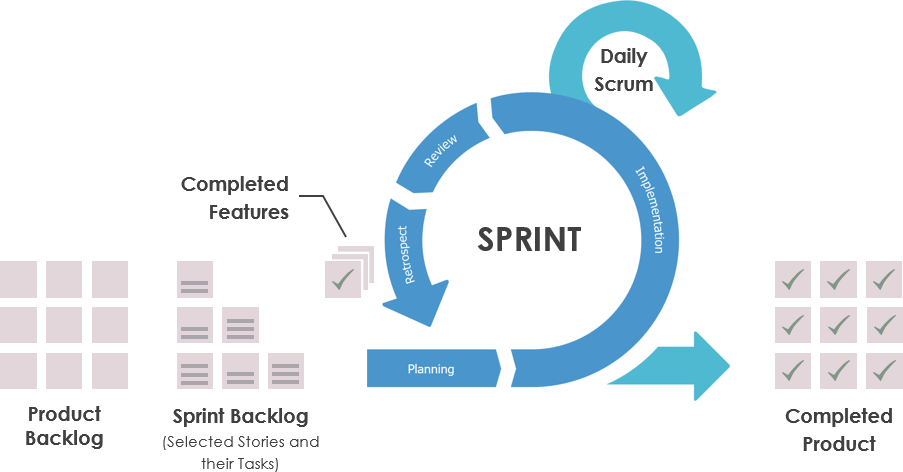
\includegraphics[width=.7\linewidth]{content/imgs/scrum_sprint.png}
  \caption{Sprint Scrum}
\end{figure}

Sur les 12 semaines de stage, sept semaines ont été consacrées au développement de l'application. J'ai donc, en début de projet, défini les fonctionnalités des sept sprints correspondant aux sept semaines. Les premières semaines ont été consacrées à la prise en main du sujet, aux recherches, à l'élaboration du cahier des charges et à la conception de l'architecture de l'application. Les deux dernières semaines ont été réservées au déploiement final de l'application sur le \textit{Play Store} et à ce rapport.

Ce planning a été modifié au cours du projet en fonctions des tâches effectivement réalisées et en fonction des imprévus.

\subsection{Gestion de versions (git)}

J'ai choisi d'utiliser le système de gestion de versions \textit{Git} avec le service d'hébergement \textit{Github} afin de donner un accès rapide et complet au travail effectué sur l'application à mon enseignant-référent et à ma tutrice de stage.

\textit{Github} m'a aussi permis de créer des points de sauvegarde du projet, appelés \textit{release}, permettant de télécharger le code source des versions majeures de l'application avec le fichier d'installation pour les appareils Android. Les \textit{releases} sont aussi accompagnées d'une description de ce qui a changé depuis la dernière version (voir l'annexe \ref{appendix:release}, exemple de la dernière \textit{release} du projet).











% eof
